\documentclass[conf]{new-aiaa}
%\documentclass[journal]{new-aiaa} for journal papers
\usepackage[utf8]{inputenc}

\usepackage{graphicx}
\usepackage{amsmath}
\usepackage{commath}
\usepackage[version=4]{mhchem}
\usepackage{siunitx}
\usepackage{longtable,tabularx}
\usepackage{float}
\usepackage{listings}
\usepackage{pdfpages}
\usepackage{color} %red, green, blue, yellow, cyan, magenta, black, white
\definecolor{mygreen}{RGB}{28,172,0} % color values Red, Green, Blue
\definecolor{mylilas}{RGB}{170,55,241}
\setlength\LTleft{0pt} 

\lstset{language=Matlab,%
	basicstyle=\footnotesize,
	breaklines=true,%
	morekeywords={matlab2tikz},
	keywordstyle=\color{blue},%
	morekeywords=[2]{1}, keywordstyle=[2]{\color{black}},
	identifierstyle=\color{black},%
	stringstyle=\color{mylilas},
	commentstyle=\color{mygreen},%
	showstringspaces=false,%without this there will be a symbol in the places where there is a space
	numbers=left,%
	numberstyle={\tiny \color{black}},% size of the numbers
	numbersep=9pt, % this defines how far the numbers are from the text
	emph=[1]{for,end,break},emphstyle=[1]\color{red}, %some words to emphasise
	%emph=[2]{word1,word2}, emphstyle=[2]{style},    
}

% ================================================================ % 
\title{ASE 389P.4 Methods of Orbit Determination \\ Homework 4: Reference Frames Transformations}

\author{Junette Hsin}
\affil{Masters Student, Aerospace Engineering and Engineering Mechanics, University of Texas, Austin, TX 78712}

\begin{document}

\maketitle

\begin{abstract}
	The transformation between an Earth	Centered Earth Fixed Earth frame and an Earth Centered Inertial frame is investigated. 


\end{abstract}


% ================================================================ % 
\section*{Problem}

 % \subsubsection*{Statement} 
\begin{center}
\fbox{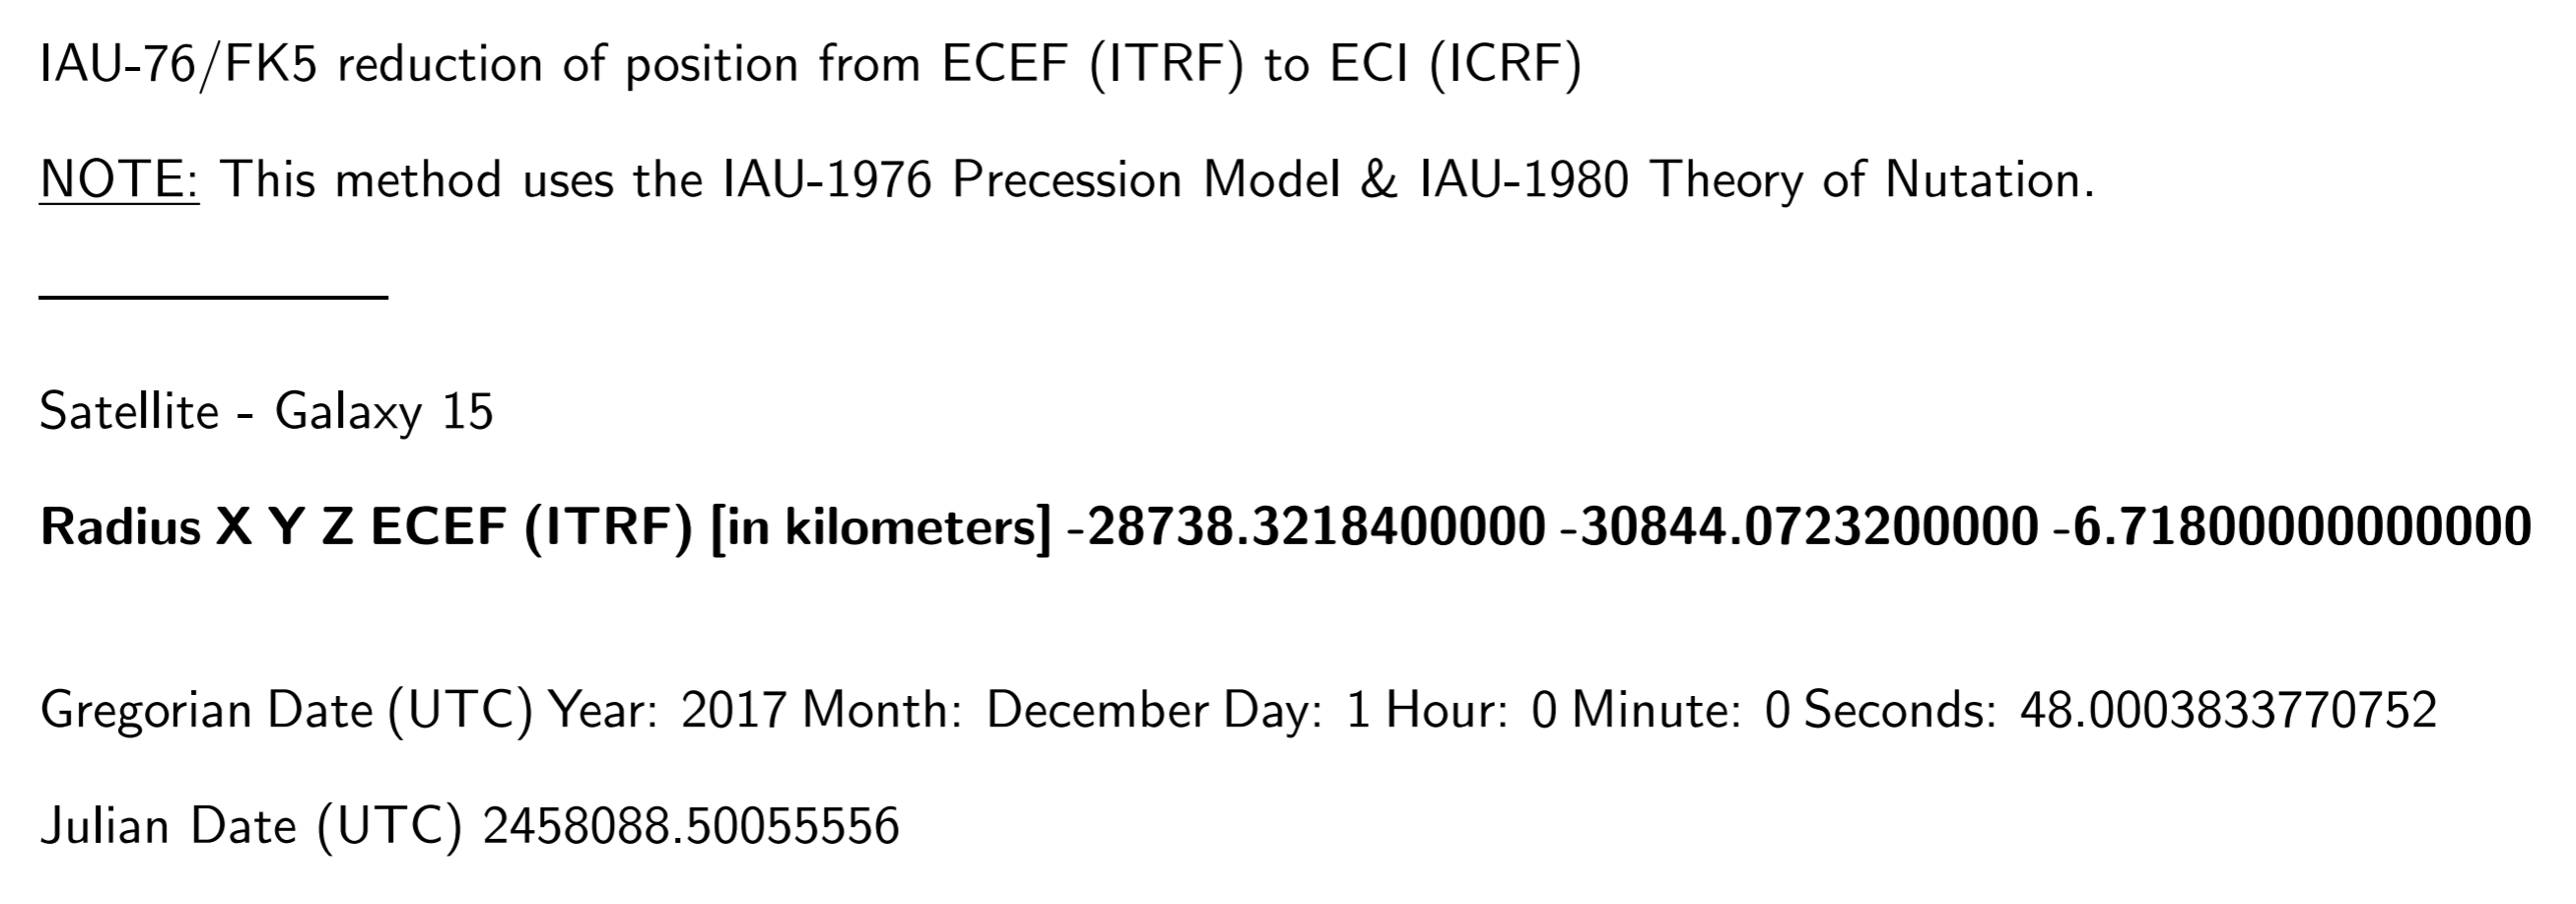
\includegraphics[width=0.9\textwidth]{prob_1.png}} \\
\end{center}

% ---------------------------------------------------------------- % 
\subsubsection*{Solution} 

The calculated position of Galaxy 15 in the ECI (ICRF) frame is: 

\begin{equation}
r\_ECI = 
\begin{bmatrix}
19165.4459607782  \\
-37549.0609887574 \\
-41.0436103252059
\end{bmatrix} 
km 
\end{equation}

The algorithm for transforming from ECEF to ECF frames was taken from Appendix H in Statistical Orbit Determination\cite{born_statorbitdet} (Born). 

\begin{equation}
T^{ECEF}_{ECI} = W S' N P 
\end{equation} 

$T^{ECEF}_{ECI}$ describes a transformation from the ECI to the ECEF frame. Transposing this matrix will result in a transformation matrix from ECEF to ECI frame. 

\begin{itemize}
	\item W is the offset of the Earth's angular velocity with respect to the z axis of ECEF. 
	\item S' is the rotation of ECEF about the angular velocity vector. 
	\item N is the nutation of ECEF with respect to ECI. 
	\item P is the precession of ECEF with respect to ECI. 
\end{itemize}

The content for the matrices W, S', and P were taken from Born. Fundamentals of Astrodynamics and Applications (Vallado) was used to calculate the nutation angles for the nutation matrix \cite{vallado}. The Errata was used to correct the Delaunay parameters in the 4th edition of the text \cite{errata}. Another resource, Satellite Orbits: Models, Methods and Applications, was used to verify the calculation of the nutation angles \cite{sat_orbits}. The IERS website was used for obtaining Earth orientation parameters (EOP) data related to the IAU1980 nutation theory \cite{iers}. The \texttt{finals.all} file was used in particular from the IERS website. 

The final satellite position in the ECI frame was within  0.000912786660221945 km, or approximately 0.913 meters of the solution given by Dr. Jah ([19165.44514777874, -37549.06140374086, -41.043609948282580] km). 

\newpage
% ================================================================ % 
\section*{Appendix} 

\subsection*{HW4 MATLAB code} 

\begin{lstlisting}[basicstyle=\footnotesize]
% HW 4

eop_data = load('finals_iau1980.txt'); 

r_ECEF  = [ -28738.3218400000; -30844.0723200000; -6.71800000000000 ];
JD      = 2458088.50055556; 

[r_ECI] = fn.ECEFtoECI(eop_data, JD, r_ECEF); 

s_vec = [19165.44514777874 -37549.06140374086 -41.043609948282580]'; 
vdiff = r_ECI - s_vec; 
\end{lstlisting}

\subsubsection{ECEFtoECI.m}

\begin{lstlisting}
function [r_ECI] = ECEFtoECI(eop_data, JD, r_ECEF)
% ------------------------------------------------------------------------ 
% Purpose: Convert ECF (ECEF/ITRF) position to ECI (ICRF) position 
% 
% Inputs: 
%   eop_data = IAU1980 EOP data (finals.all)
%   JD       = Julian Date (UTC) 
%   r_ECEF   = position in ECEF (Earth-centered Earth-fixed) frame
% 
% Outputs: 
%   r_ECI    = position in ECI (Earth-centered inertial) frame 
% 
% References: 
%   Statistical Orbit Determination by Bob E. Schutz, George Born, and Tapley
% 
% Notes: 
%   Transformation to ECI from ECEF: 
%   ECI_DCM_ECEF = W * S' * N * P; 
%   W  = offset of Earth's angular velocity vector wrt ECEF Z axis 
%   S' = rotation of ECF about angular velocity vector 
%   N  = nutation of ECF wrt ECI 
%   P  = precession of ECF wrt ECI 
% ------------------------------------------------------------------------ 

% P  = precession of ECF wrt ECI 
P = fn.precession(JD); 

% N  = nutation of ECF wrt ECI  
[N, em, dpsi] = fn.nutation(JD); 

% S' = rotation of ECF about angular velocity vector 
[xp, yp, dT] = fn.iers_data(eop_data, JD); 
GSMT = 4.894961212823058751375704430 + dT * ... 
( 6.300388098984893552276513720 + dT * ... 
( 5.075209994113591478053805523e-15 - ... 
-9.253097568194335640067190688e-24 * dT) ); 

aG = GSMT + dpsi * cos(em); 
Sp = [cos(aG), sin(aG), 0; -sin(aG), cos(aG), 0; 0, 0, 1 ]; 

% W  = offset of Earth's angular velocity vector wrt ECEF Z axis 
W = [1 0 xp; 0 1 -yp; -xp yp 1]; 

% ECI position calculation 
ECI_C_ECEF = (W * Sp * N * P)'; 
r_ECI      = fn.orthodcm(ECI_C_ECEF) * r_ECEF; 

end 
\end{lstlisting}

\subsubsection{precession.m }
\begin{lstlisting}
function P = precession(JD) 

t   = (JD - 2451545.0)./36525;

% precession angles ... in arcseconds 
zeta  = 2306.2181 * t + 0.30188 * t^2 + 0.017998 * t^3; 
theta = 2004.3109 * t - 0.42655 * t^2 - 0.041833 * t^3; 
z     = 2306.2181 * t + 1.09468 * t^2 + 0.018203 * t^3; 

% convert arcsec --> deg --> rad 
zeta  = zeta/3600 * pi/180; 
theta = theta/3600 * pi/180; 
z     = z/3600 * pi/180; 

% P row 1 coeffs 
p11 = cos(zeta)*cos(theta)*cos(z) - sin(zeta)*sin(z); 
p12 = -sin(zeta)*cos(theta)*cos(z) - cos(zeta)*sin(z); 
p13 = -sin(theta)*cos(z); 

% P row 2 coeffs 
p21 = cos(zeta)*cos(theta)*sin(z) + sin(zeta)*cos(z); 
p22 = -sin(zeta)*cos(theta)*sin(z) + cos(zeta)*cos(z); 
p23 = -sin(theta)*sin(z); 

% P row 3 coeffs 
p31 = cos(zeta)*sin(theta); 
p32 = -sin(zeta)*sin(theta); 
p33 = cos(theta); 

% P  = precession of ECF wrt ECI 
P = [ p11, p12, p13 ; 
p21, p22, p23 ; 
p31, p32, p33 ]; 

end
\end{lstlisting}

\subsubsection{nutation.m}
\begin{lstlisting}
function [N, em, dpsi] = nutation(JD)

% time = number of centuries since J2000 as terrestrial time (TT) 
t   = (JD - 2451545.0)./36525;
MJD = JD - 2400000.5; 

%% N  = nutation of ECF wrt ECI 

% em    = mean obliquity of the ecliptic 
% et    = true obliquity of the ecliptic 
% dpsi  = nutation in longitude 
% de    = nutation in obliquity 

% mean obliquity 
em = 84381.448 - 46.8150 * t - 0.00059 * t^2 + 0.001813 * t^3; 
em = em/3600 * pi/180; 

% nutation in longitude and obliquity ????? 
[dpsi, de] = fn.nut_angles(JD);

% true obliquity 
et = em + de; 

n11 = cos(dpsi); 
n12 = -cos(em) * sin(dpsi); 
n13 = -sin(em) * sin(dpsi); 

n21 = cos(et) * sin(dpsi);
n22 = cos(em) * cos(et) * cos(dpsi) + sin(em) * sin(et); 
n23 = sin(em) * cos(et) * cos(dpsi) - cos(em) * sin(et); 

n31 = sin(et) * sin(dpsi); 
n32 = cos(em) * sin(et) * cos(dpsi) - sin(em) * cos(et); 
n33 = sin(em) * sin(et) * cos(dpsi) + cos(em) * cos(et); 

N = [n11 n12 n13; n21 n22 n23; n31 n32 n33]; 

end
\end{lstlisting}

\subsubsection{nut\_angles.m}
\begin{lstlisting}
function [dpsi, deps] = nut_angles(JD)

% JD_TT = Mjd_TT + 2400000.5; 
MJD = JD - 2400000.5; 
T   = (MJD - 51544.5)/36525;
rev = 360;  % deg/revoluton 

C = load('nut80.dat'); 
C(:, 6:end) = C(:, 6:end)*10; 

% From errata: Delaunay parameters, mean arguments of luni-solar motion in deg
%   Mm = mean anomaly of the Moon
%   Ms = mean anomaly of the Sun
%   uM = mean argument of latitude
%   D  = mean longitude elongation of the Moon from the Sun 
%   Om = mean longitude of the ascending node  
Mm = 134.96298139 + ( 1325*rev + 198.8673981 )*T + 0.0086972*T^2 + 1.78e-5*T^3; 
Ms = 357.52772333 + ( 99*rev   + 359.0503400 )*T - 0.0001603*T^2 - 3.3e-6*T^3; 
uM = 93.27191028  + ( 1342*rev + 82.0175381  )*T - 0.0036825*T^2 + 3.1e-6*T^3; 
D  = 297.85036306 + ( 1236*rev + 307.1114800 )*T - 0.0019142*T^2 + 5.3e-6*T^3; 
Om = 125.04452222 - ( 5*rev    + 134.1362608 )*T + 0.0020708*T^2 + 2.2e-6*T^3; 

% Nutation in longitude and obliquity 
dpsi = 0;
deps = 0;

for i = 1:length(C)
api  =  ( C(i,1) * Mm + C(i,2) * Ms + C(i,3) * uM + C(i,4) * D + C(i,5) * Om ) * pi/180;
dpsi = dpsi + ( C(i,6) + C(i,7) * T ) * sin(api);
deps = deps + ( C(i,8) + C(i,9) * T ) * cos(api);
end

dpsi = 1e-5 * dpsi / 3600 * pi/180;
deps = 1e-5 * deps / 3600 * pi/180;

end
\end{lstlisting}

\subsubsection{iers\_data.m}
\begin{lstlisting}
function [xp_rad, yp_rad, dT] = iers_data(eop_data, JD) 
% From Bulletin A: 
% 
% 1         2       3       4       5       6       7       8       
% year      month   day     MJD     xp      dxp     yp      dyp 
% 
% 9         10      11      12      13      14      15      16 
% UT1-UTC   d       LOD     dLOD    dPsi    ddPsi   deps    ddeps 
%           UT1-UTC         

% From Bulletin B: 
% 17        18          19          20                  21      
% PM x asec PM y asec   UT1-UTC (s) dPsi (milli asec)   deps (milli asec) 

%% get xp, yp 

% Modified JD 
MJD = JD - 2400000.5; 

% find day 
mjd_day = floor(MJD); 

% day fraction 
dfrac = (MJD - mjd_day) / 86400; 

% find MJD row 
i_row = find(eop_data(:,4) == mjd_day, 1, 'first');  

% interpolate 
xp1_asec = eop_data(i_row, 5); 
xp2_asec = eop_data(i_row + 1, 5); 
xp_asec  = (xp2_asec - xp1_asec) * dfrac + xp1_asec; 

yp1_asec = eop_data(i_row, 7); 
yp2_asec = eop_data(i_row + 1, 7); 
yp_asec  = (yp2_asec - yp1_asec) * dfrac + yp1_asec; 

xp_rad   = xp_asec / 3600 * pi/180; 
yp_rad   = yp_asec / 3600 * pi/180; 

%% get dT 

% julian day for Jan 1, 2000 12:00 TT: 2451545
% UT1 = JD + dUT1_UTC 
% dT = UT1 - 2451545 

% interpolate 
dUT1 = eop_data(i_row, 9) / 86400; % seconds --> days  
dUT2 = eop_data(i_row+1, 9) / 86400; % seconds --> days  
dUT = (dUT2 - dUT1) * dfrac + dUT1; 

UT1 = JD + dUT; 
dT = UT1 - 2451545; 

end 
\end{lstlisting}


% ================================================================ % 

s\bibliography{sample}

\end{document}
